\documentclass[addpoints]{exam}
\usepackage[utf8]{inputenc}
\usepackage[portuguese]{babel}
\usepackage[LGRgreek]{mathastext}
\usepackage{graphicx,graphics}
\usepackage{hyperref}
\usepackage{framed}
\usepackage{multirow}
\usepackage{booktabs}

\footer{}{\thepage}{}

\renewcommand{\arraystretch}{1.3}
%\setlength{\tabcolsep}{pt}
 
\pointpoints{ponto}{pontos}
\bonuspointpoints{ponto extra}{pontos extra}
 
\totalformat{Pregunta \thequestion: \totalpoints pontos}
 
\chqword{Pregunta}
\chpgword{Página}
\chpword{Pontos}
\chbpword{Pontos extra}
\chsword{Pontos obtidos}
\chtword{Total}

\hqword{Questão}
\hpgword{Página}
\hpword{Pontos}
\hsword{Pontos obtidos}
\htword{Total}

 
\begin{document}
 
\large

\begin{center}
\Large
\textbf{Laboratório de Eletrônica Básica II – EE641}
\end{center}

\normalsize
 
\vspace{5mm}
 

 
\noindent\makebox[0.72\textwidth]{Nome: \enspace\hrulefill}
\hfill
\makebox[0.2\textwidth]{RA: \enspace\hrulefill}

\vspace{5mm}

\noindent\makebox[0.72\textwidth]{Nome: \enspace\hrulefill}
\hfill
\makebox[0.2\textwidth]{RA: \enspace\hrulefill}

\vspace{5mm}

\noindent\makebox[0.72\textwidth]{Nome: \enspace\hrulefill}
\hfill
\makebox[0.2\textwidth]{RA: \enspace\hrulefill}

\vspace{5mm}

\noindent\makebox[0.72\textwidth]{Nome: \enspace\hrulefill}
\hfill
\makebox[0.2\textwidth]{RA: \enspace\hrulefill}

\vspace{5mm}

\noindent\makebox[0.72\textwidth]{Nome: \enspace\hrulefill}
\hfill
\makebox[0.2\textwidth]{RA: \enspace\hrulefill}


%\begin{center}
%\gradetable[h][questions]
%\end{center}

\vspace{2mm}


\begin{center}
\large
\textbf{REALIMENTAÇÃO}
\normalsize
\end{center}

\begin{questions}

\section*{Fonte de corrente para LEDs}

\question Monte o circuito ``Fonte de corrente para LEDs'' da Figura \ref{cir:1} na \textbf{protoboard}. Utilize uma fonte de alimentação VCC = 30 V. Projete os valores de R1, R2 e Rshunt de maneira que I(Rshunt) = 10 mA, V(Rshunt) $\le$ 0,5 V e I(R1) $\le$ 100 $\mu$A. Efetue os cálculos e os mostre no espaço abaixo.
\label{part:a}

\begin{figure}[h!]
\begin{center}
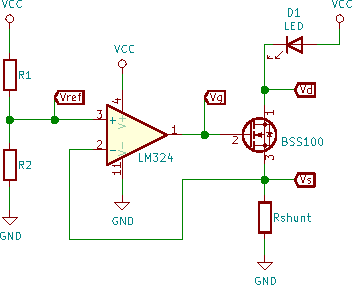
\includegraphics[width=0.4\textwidth]{imagens/realimentacao.pdf}
\end{center}
\caption{Fonte de corrente para LEDs.}
\label{cir:1}
\end{figure}

\begin{framed}
\vspace{4cm}
\end{framed} 

\pagebreak

\begin{parts}

\part (PÓS EXPERIMENTO) Explique o funcionamento do circuito do item (\ref{part:a}).
\begin{framed}
\vspace{3cm}
\end{framed} 

\part Com o circuito do item (\ref{part:a}), varie o número de LEDs, dispondo-os em série, e complete a Tabela \ref{tab:1}:

\begin{table}[h!]
\centering
\begin{tabular}{|c|c|c|c|c|c|c|c|c|}
\hline
\textbf{\# LEDs} & \textbf{R1 [k$\Omega$]} & \textbf{R2 [k$\Omega$]} & \textbf{Rshunt [$\Omega$]} & \textbf{Vref [V]} & \textbf{Vs [V]} & \textbf{Vd [V]} & \textbf{Vg [V]} & \textbf{Pot(Q1) [mW]} \\ \hline
1 &  &  &  &  &  &  &  &  \\ \hline
2 &  &  &  &  &  &  &  &  \\ \hline
3 &  &  &  &  &  &  &  &  \\ \hline
\end{tabular}
\caption{Tensões ao longo do circuito.}
\label{tab:1}
\end{table}

\part (PÓS EXPERIMENTO) Identifique no diagrama de controle abaixo cada elemento do circuito montado no item (\ref{part:a}):
\label{part:b}
\begin{framed}

\begin{center}
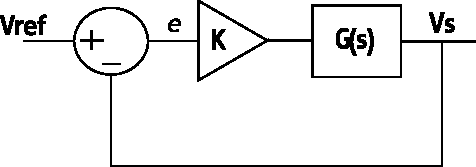
\includegraphics[width=0.4\textwidth]{imagens/controle.pdf}
\end{center}
\vspace{9.5cm}
\end{framed}

\pagebreak

\part (PÓS EXPERIMENTO) Para o sistema do item (\ref{part:b}):
\begin{subparts}
\subpart O que acontece com o erro \textit{e} e com a relação Vref/Vs se $K \rightarrow \infty$? Mostre matematicamente a partir da função de transferência de malha fechada. 
\subpart Relacione sua resposta com os valores de tensão encontrados entre as portas inversora e não-inversora do LM324, resumidos na Tabela \ref{tab:1}. 
\end{subparts}
\begin{framed}
\vspace{7cm}
\end{framed}
\end{parts}

\section*{Regulador de tensão linear}

\question Para o circuito ``Regulador de tensão linear'' da Figura \ref{cir:2}, projete o valor de Rzener para devida polarização do diodo zener de 2,5 V. Selecione os componentes Cin = 0.47 mF, Cout = 100 nF, Rload = 100 k$\Omega$ e monte o circuito na \textbf{protoboard}.
\begin{framed}
Rzener = 
\end{framed}

\begin{figure}[h!]
\begin{center}
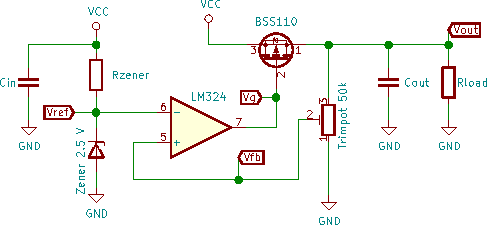
\includegraphics[width=0.7\textwidth]{imagens/realimentacao2.pdf}
\end{center}
\caption{Regulador de tensão linear.}
\label{cir:2}
\end{figure}

\pagebreak

\begin{parts}
\part Varie o trimpot de tal modo a atingir os valores de Vout da Tabela \ref{tab:2}. Complete os itens faltantes.
\begin{table}[h!]
\centering
\begin{tabular}{|c|c|c|c|c|c|c|c|c|}
\hline
\textbf{Vout [V]} & \textbf{Vref [V]} & \textbf{Vfb [V]} & \textbf{Vg [V]}  \\ \hline
5 	&  &  &   \\ \hline
18 	&  &  &   \\ \hline
24 	&  &  &   \\ \hline
\end{tabular}
\caption{Tensões ao longo do circuito.}
\label{tab:2}
\end{table}

\part (PÓS EXPERIMENTO) Baseado em um diagrama de blocos de um regulador de tensão linear, identifique os elementos do circuito que fazem parte de um circuito integrado comercial.
\begin{framed}
\vspace{10cm}
\end{framed}
\part (PÓS EXPERIMENTO) Qual a funcionalidade dos capacitores Cin  e Cout?
\begin{framed}
\vspace{3cm}
\end{framed}

\pagebreak
\part (PÓS EXPERIMENTO) Se é possível fabricar capacitores em circuito integrado, por que tipicamente Cin e Cout são dispostos externamente no chip? Comente sobre a relação entre área no \textit{wafer} de semicondutor, custo de produção e valores de capacitância.
\begin{framed}
\vspace{7cm}
\end{framed}
\end{parts}


\vspace{5mm}


\end{questions}

\end{document}
